\documentclass{article}

% По возможности эту строчку необходимо добавить сразу же после команды \documentclass. 
% В этом случае для всех остальных загружаемых пакетов будет использоваться выбранный язык. 
% Список языков, подключаемых в установленной у Вас системе LaTeX, отображается при каждой компиляции документа. 
% Если установленный Вами формат LaTeX не поддерживает расстановку переносов выбранного языка, 
% то пакет babel будет продолжать свою работу, отключив расстановку переносов. 
% Это отрицательно скажется только на внешнем виде документа.

\usepackage[english, russian]{babel}
% Правильное отображение стилей
\usepackage[T2A]{fontenc}
\usepackage[utf8]{inputenc}
% Точка вместо двоеточия в подписях картинок
\usepackage[labelsep=period]{caption}
% Установка междустрочных интервалов
\usepackage{setspace}
% Изменение положения рисунков относительно текста
\usepackage{float}


% Изменение построения элементов заголовка
\makeatletter
\renewcommand\@maketitle{%
  \newpage
  \null
  \vskip 2em%
  \begin{center}%
  \let \footnote \thanks
    {\large
      \lineskip .5em%
      \begin{tabular}[t]{c}%
        \@author
      \end{tabular}\par}%
    \vskip 1.5em%
    {\LARGE \@title \par}%
    \vskip 2.5em%
    {\large \@date}%
  \end{center}%
  \par
  \vskip 1.5em}
\makeatother


% Размеры страницы
\usepackage[a4paper,top=2cm,bottom=3cm,left=2.5cm,right=2.5cm,marginparwidth=1.75cm]{geometry}

% Подпись к картинкам курсивом
\usepackage[format=plain,
            font=it]{caption}

% Убрать дефолтное слово "Аннотация"
\addto{\captionsrussian}
{\renewcommand{\abstractname}{}}

% Математика и ссылки
\usepackage{amsmath}
\usepackage{graphicx}
\usepackage[colorlinks=true, allcolors=blue]{hyperref}

\linespread{0.75}
\title{\vspace{-1ex}\textbf{\large РАЗРАБОТКА АЛГОРИТМА ОБУЧЕНИЯ ИНТЕЛЛЕКТУАЛЬНОЙ
СИСТЕМЫ УПРАВЛЕНИЯ НА ОСНОВЕ ГЕНЕТИЧЕСКИХ
АЛГОРИТМОВ}}
\date{\vspace{-10ex}}
\author{\textbf{\normalsize И.С. Коберси, В.В. Шадрина}}


\begin{document}

\maketitle

\linespread{1}
\begin{abstract}
    \textit{\normalsize Рассмотрена разработка генетического алгоритма для обучения интеллектуальной системы управления транспортными средствами, система управления является нейро-нечеткой.\\\indent Нейронная система; генетические алгоритмы.}
\end{abstract}

  \onehalfspace {
  \large \textrm{\indent Нечеткая логика позволяет строить карты входного пространства вплоть до выходного пространства. 
Механизм построения выполняется посредством формирования правил IF-THEN, для этого необходимо тщательно построить нечеткие правила и их набор \cite{rutkovskaya2008nejronnye}.
Основная проблема состоит в том, что применение данного подхода представляет некоторую трудность построения функции принадлежности.
Генетический алгоритм -- это технология, которая эмулирует теорию эволюции для решений сложных задач оптимизации. Генетические алгоритмы представляют 
альтернативу традиционным методам оптимизации, с применением случайного поиска, чтобы получить набор оптимальных решений. Генетические алгоритмы буквально ищут 
относительно двух концов пространства поиска с тем, чтобы определить оптимизационное решение. Популяции всех решений оцениваются для определения наилучшего решения.
Гибридная система комбинирует систему нейронного нечеткого интерфейса, а генетические алгоритмы применяются для настройки параметров гибридной сети (ННС). Цель 
заключается в сокрушении набора правил, прежде чем подавать на вход сети. Модификации, внесенные в разные (отдельные) слои сети, повышают ее производительность.
Предложенный ГА ННС-сети в состоянии достичь высоких классификационных показателей по сравнению с ННС-сетей. На рис. 1 показана гибридная система управления 
транспортными средствами ТС, она состоит из трех основных модулей.\\
\indent В этой статье рассматривается разработка модуля управления скоростью ТС.}\\ 
}
\begin{center}\vspace{-3ex}
\textbf{Архитектура модуля управления скоростью ТС}\\
\end{center}
\indent\indent \large Слои характеризуются нечеткими операциями по следующему порядку:
\begin{itemize}\vspace{-1ex}
    \setlength\itemsep{-0.3em}
    \large
    \item первый слой (входной слой);
    \item второй слой (слой состояний);
    \item третий слой (правило -- базовый слой);
    \item слой четвертый (слой отбора правил);
    \item пятый слой (слой следствия);
    \item шестой слой (выходной слой).
  \end{itemize}

  % Помещение картинки в начало страницы
  \makeatletter
  \setlength{\@fptop}{0pt}
  \makeatother
% Даёт подпись после картинки
  \clearpage

  \begin{figure}
    \centering
    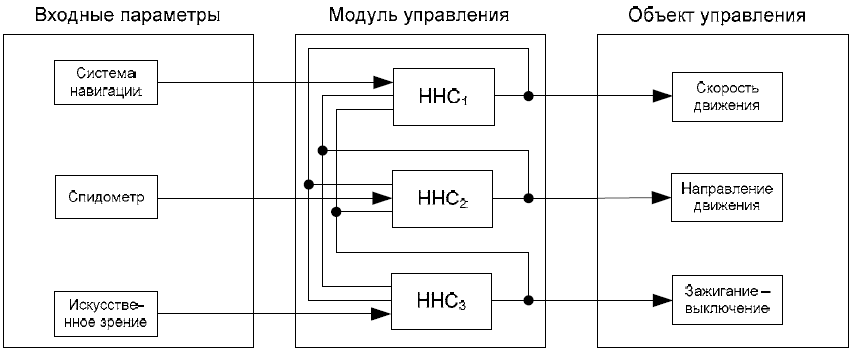
\includegraphics[width=1\textwidth]{Figures/pic_1.png}
    \caption{\label{fig:scheme}Модуль системы управления транспортными средствами}
  \end{figure}
  \onehalfspace { 
  \indent\indentКаждый слой имеет свое число нейронов. Число нейронов каждого слоя упорядочено. Номер нейронов в k-м слое назовем $N_{k}$,
  где $k \in \{1,\ldots, 6\}$. Нейроны, расположенные в k-м слое, имеют связь E. Значение $E_{i,j}^k$ означает связь i-го нейрона
  k-1-слоя с j-м нейроном k-го слоя, где $k \in \{2,\ldots, 6\}, i \in \{1,\ldots, N_{k-1}\}$ и $j \in \{1,\ldots, N_k\}$. 
  Это не означает связь двух нейронов одного и того же слоя. Связи в нейронных сетях содержат веса w. 
  В модуле [1,2] значения всех весов связей встраиваются вместе с нейронами. Таким образом, веса связи $E_{i,j}^k$ обозначаются
  $w_{i,j}^k$ и соединены с j-ми нейронами k-го слоя. \\\indent\indent\textbf{Первый слой (I) – входной слой.} Вход модуля является ненечетким 
  вектором данных, представляющим собой $\vec{x}=[x_1,x_2,x_3,\ldots,x_i,\ldots,x_{N_{1}}]^T$. Функция этого слоя заключается в приеме 
  входных параметров, преобразовании их в одиночные нечеткие множества и передаче на следующий слой. Узлы (переменные)в этом слое 
  называются лингвистическими переменными; они представляют входные лингвистические переменные типа “скорость”, “направление”, 
  “препятствие” и т.д.\\\indent\indent Однако в этой актуальной реализации все входы принимают non-нечеткие векторные значения. 
  Следовательно, процесс non-фаззификации выполняется. Лингвистические связи прямо соединяют (передают) non-нечеткие входы на 
  следующий слой. Каждый узел принимает только один вход в качестве одного из аспектов входных векторных данных по всей сети и 
  вывод на несколько узлов следующего слоя.\\\indent\indent Функции входа и вывода определяются следующими формулами:
  }
  \begin{center}
    {
      Net вход: $f_i^I=x_i$ для $i=1,\ldots,N_1,$\\
      Net вывод: $o_i^I=f_i^I$ для $i=1,\ldots,N_1,$\\
    }
  \end{center}
  {
    где $f_i^I$ -- вход узла i в (первом) слое I; $o_i^I$ -- вывод узла i в слое I; и $x_i$ -- i-й элемент входного вектора $\vec{x}$.\\
  \indent\indent\textbf{Второй слой (II) – слой состояний.} Нейроны этого слоя называются узлами ввода элементов. Они представляют 
  собой такие переменные как “высокий”, “средний” или “медленный” из соответствующих входных лингвистических переменных. 
  Подобная структура показана на рис. 2.
  }
  \begin{figure} [H]
    \centering
    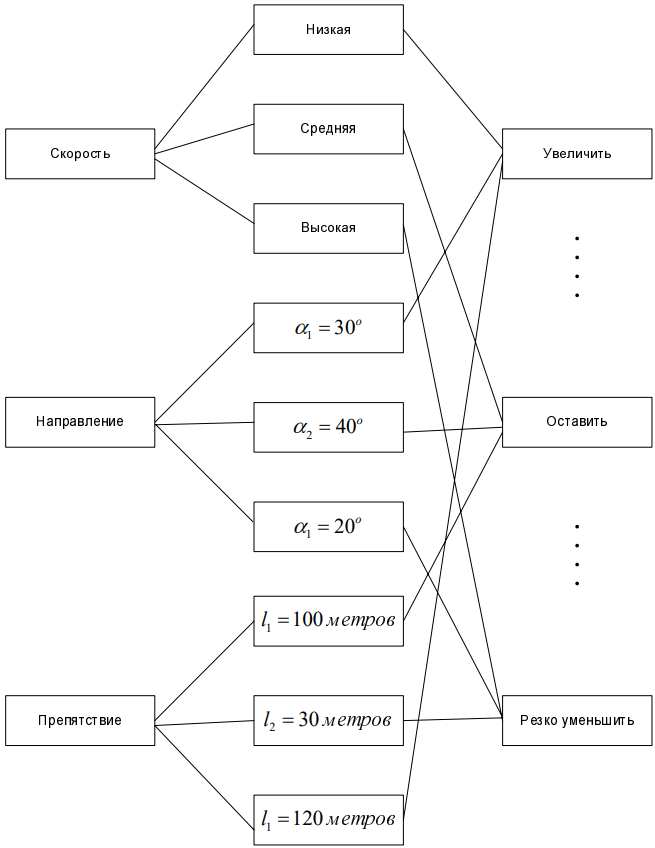
\includegraphics[width=1\textwidth]{Figures/pic_2.png}
    \caption{\label{fig:block-scheme}Иллюстрация простого примера интерфейса нечеткого управления}
  \end{figure}
  {
  \indent\indent\indent Показные значения на рис. 2 “скорость”, “направление” и “препятствие” представляют собой лингвистические переменные трех 
  терм множества входного слоя. А девять узловых значений в слое состояний (второй слой), представляют “состояние скорости”, 
  “состояние направления” и “состояние препятствия”.\\
  \indent\indent Входные значения применяют значения IL. Значения $IL_{i,j}$ обозначают узловые соединения j-го значения i-й 
  входной лингвистической переменной.\\
  \indent\indent Каждое входное узловое значение имеет только один вход, но с его выхода можно передать один или более выводов на следующий слой. 
  Каждый узел этого слоя имеет одну функцию принадлежности. Аргумент выбора функции принадлежности исходит от подключенного 
  лингвистического узла в первом слое. Выходные значения входного узлового слоя представляют собой значение принадлежности.\\
  \indent\indent Часто применяемая функция принадлежности имеет трапецеидальную форму, но в нашем случае применяется треугольная 
  форма, поскольку данная функция имеет два боковых ограничения и один центр, в отличие от общепринятой формы, которая имеет 
  четыре боковых и ни одного центра.\\
  \indent\indent Горизонтальная ось функции принадлежности представляет собой входные лингвистические значения, 
  а вертикальные оси представляют значения функции принадлежности $\mu(x_i)$, где $x_i$ –- параметр i-й лингвистической 
  переменной и $\mu(x_i) \in [0,1]$. На рис. 3 показан вид функции принадлежности \cite{finaev2005modeli}.
  }
  \begin{figure} [H]
    \centering
    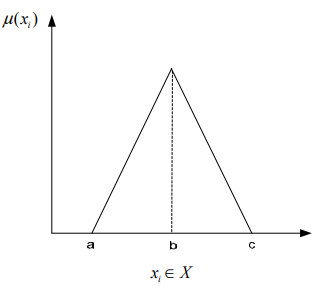
\includegraphics[width=0.5\textwidth]{Figures/pic_3.png}
    \caption{\label{fig:chart}Треугольная функция принадлежности}
  \end{figure}
  {
    \indent\indent\indent Входное значение узла $IL_{i,j}$ обозначает j-е значение i-й лингвистической переменной, вход и выход функции 
    заданы следующими формулами:\\
  }
  \begin{center}
    \Large
    $$\text{вход }f_{ij}^{II}=
    \begin{cases}
      0, x \in [-\infty, a_i^k],\\
      \frac{x_i - a_i^k}{b_i^k - a_i^k}, x \in [a_i^k, b_i^k],\\
      \frac{x_i - c_i^k}{b_i^k - c_i^k}, x \in [a_i^k, c_i^k],\\ 
      0, x \in [c_i^k, +\infty],
    \end{cases}$$
  \end{center}
  {
    для $i = 1, \ldots, N_1$ и $j = 1, \ldots, N_2$,
  }
  \begin{center}
    $f_{ij}^{II}=o_{ij}^{II}$ для $i=1,\ldots,N_1$ и $j=1,\ldots,N_2$.
  \end{center}
  {
  \indent\indent Значение выхода: где $o_i^I$ вывод i-го лингвистического узла в первом слое и $\{a_{ij}^{II}, b_{ij}^{II}, c_{ij}^{II}\}$
  это параметры треугольной функции принадлежности.\\
  \indent\indent \textbf{Третьи слой (III) – слой базы правил.} Этот слой определяет нечеткие правила. Каждый его нейрон включает 
  в себя нечеткие правила и называется узлом правил. Любая функция этого слоя узловых правил может быть проиллюстрирована, 
  как показано на рис. 3.\\
  }
  \begin{center}
    \textbf{ЕСЛИ} ТС едет со скоростью $\nu_1$ , \textbf{И ЕСЛИ} ТС двигается под углом $\alpha_1$,\\
    \textbf{И ЕСЛИ} обнаружено препятствие $\rho_1$ , \textbf{ТО} изменить скорость на значение $\nu_1\pm\nu_i$.
    \textbf{ЕСЛИ} ТС едет со скоростью $\nu_2$ , \textbf{И ЕСЛИ} ТС двигается под углом $\alpha_2$,\\
    \textbf{И ЕСЛИ} обнаружено препятствие $\rho_2$ , \textbf{ТО} изменить скорость на значение $\nu_2\pm\nu_i$.
    \textbf{ЕСЛИ} ТС едет со скоростью $\nu_3$ , \textbf{И ЕСЛИ} ТС двигается под углом $\alpha_3$,\\
    \textbf{И ЕСЛИ} обнаружено препятствие $\rho_3$ , \textbf{ТО} изменить скорость на значение $\nu_3\pm\nu_i$.
  \end{center}
  {
    \indent\indent Слова “увеличить”, “оставить” и “резко увеличить скорость” –- это соответствующие узловые правила. 
    Число выводов каждого узлового правила фиксировано-единственно, но число входов каждого узлового правила не фиксировано, 
    а входит в интервал от 1 до $N_1$ (количество входной размерности) в зависимости от количества нечетких правил.\\
    \indent\indent Количества входных и выходных функций k-го узлового правила этого слоя определяются следующими функциями соответственно:
  }
  \begin{center}
    входы: $f_l^{IV}=o_k^{III}$ для $l=1,\ldots,N_4$,\\
    и $k=1,\ldots,N_3$;\\
    $$\text{выходы: }o_l^{IV}=
    \begin{cases}
      1, \text{когда } f_l^{IV} \text{максимальная},\\
      \text{для } l=1,\ldots,N_4 \\
      0 \text{ иначе}
    \end{cases}$$
  \end{center}
  {
    где $o_k^{III}$ -- чистый выход k-го узлового правила в третьем (III) слое; $f_l^{IV}$ -- чистый
    вход выбранного l набора узлов четвертого слоя (IV); $o_l^{IV}$ -- чистый выход выбранного l набора узлов 
    четвертого слоя (IV).
  }
  \begin{figure} [H]
    \centering
    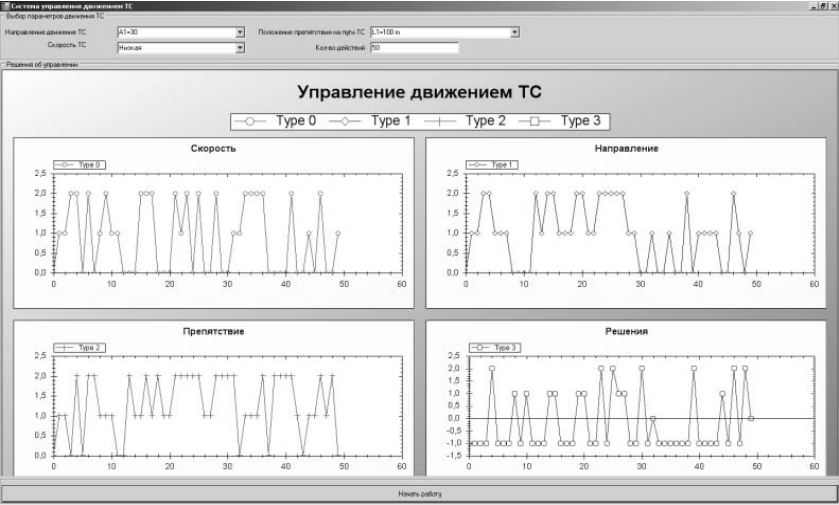
\includegraphics[width=0.5\textwidth]{Figures/pic_4.png}
    \caption{\label{fig:system}Треугольная функция принадлежности}
  \end{figure}
  {
    \indent\indent \textbf{Пятый слой (IV) – слой следствия (вывода).} Узлы этого слоя называются узлами следствия, и каждый его узел 
    имеет количество N1+1 от входного слоя, имеющего два входа: первый от предыдущего слоя и N1 (количество входных данных). 
    Первый вход от предыдущего слоя обеспечивает запуск силы связанных нечетких правил. 
    Вход и выход этого слоя определяются следующими выражениями:\\
  }
  {
    \\\indent\indent входы: $f_m^V=c_0x_0+c_1x_1+c_2x_2+\ldots+c_{N_{1}}x_{N_{1}}$, для $m=1,\ldots,N_5$,\\
    \indent\indent выходы: $o_m^V=o_m^{IV}f_m^V$ для $m=1,\ldots,N_5$,\\\\
  }
  {
    где $f_m^V$ -- чистый вход m-го определенного узла пятого слоя (V); $c_i$ -- коэффициент i-й входной переменной;
    $o_m^{IV}$ -- выходное значение m-го узла четвертого слоя (VI); $v_m^V$ -- чистое выходное значение m-го узла пятого 
    слоя (V). Значение $\{c_0,x_1,x_2,\ldots,c_i,\ldots,c_{N_{1}}\}$ представляет собой набор параметров. Упомянутые па-
    раметры этого слоя являются параметрами следствия (вывода).\\
  }
  {
    \indent\indent \textbf{Шестой слой (IV) -- выходной слой.} Этот слой содержит только один узел, и он называется узлом выхода. 
    Таким образом, значение $N_5=1$. Он суммирует все выходные значения предыдущего слоя (слой следствий).\\
    \indent\indent Функция выхода сети представляется следующим образом:
  }
  \begin{center}
    $$o^{VI}=f^{VI}=\sum_{N_5}^{m=1} o_m^V,$$
  \end{center}
  {
    где $f^{VI}$ -- чистый вход выходного узла; $o^{VI}$ -- чистый выход выходного узла; $o^V$ -- выходное значение пятого слоя (V).
  }
\bibliographystyle{abbrv}
\bibliography{Library/sample}
\end{document}